

\chapter{Analysis of Algorithms  |  算法分析}
\label{algorithms}

\begin{quote}
This appendix is an edited excerpt from {\it Think Complexity}, by
Allen B. Downey, also published by O'Reilly Media (2012).  When you
are done with this book, you might want to move on to that one.
\end{quote}

\begin{quote}
本附录摘自 Allen B. Downey的 {\em Think Complexity}, 也由 O’Reilly Media (2011)出版。 当你读完本书后,也许你可以参考这本读读。
\end{quote}

{\bf Analysis of algorithms} is a branch of computer science that
studies the performance of algorithms, especially their run time and
space requirements.  See
\url{http://en.wikipedia.org/wiki/Analysis_of_algorithms}.

{\em 算法分析} ({\bf Analysis of algorithms}) 是计算机科学的一个分支,
 着重研究算法的性能, 特别是他们的运行时间和资源开销。
见:\href{http://en.wikipedia.org/wiki/Analysis_of_algorithms}{算法分析\textsuperscript{(维基百科)}} 。
\index{algorithm} \index{analysis of algorithms}

The practical goal of algorithm analysis is to predict the performance
of different algorithms in order to guide design decisions.

算法分析的实际目的是预测不同算法的性能,用于指导设计层的决策。

During the 2008 United States Presidential Campaign, candidate
Barack Obama was asked to perform an impromptu analysis when
he visited Google.  Chief executive Eric Schmidt jokingly asked him
for ``the most efficient way to sort a million 32-bit integers.''
Obama had apparently been tipped off, because he quickly
replied, ``I think the bubble sort would be the wrong way to go.''
See \url{http://www.youtube.com/watch?v=k4RRi_ntQc8}.

2008年美国总统大选期间,当候选人 奥巴马(Barack Obama) 访问Google时,
他被要求进行即席的分析。首席执行官Eric Schmidt开玩笑的问他
``对一百万个32位整数排序的最有效的方法''。
显然有人暗中通知了奥巴马,因为他很快回答, ``我认为不应该采用冒泡排序法''。
详见\href{http://www.youtube.com/watch?v=k4RRi_ntQc8}{这个视频}。
\index{Obama, Barack}  \index{Schmidt, Eric}  \index{bubble sort}

This is true: bubble sort is conceptually simple but slow for
large datasets.  The answer Schmidt was probably looking for is
``radix sort'' (\url{http://en.wikipedia.org/wiki/Radix_sort})\footnote{
But if you get a question like this in an interview, I think
a better answer is, ``The fastest way to sort a million integers
is to use whatever sort function is provided by the language
I'm using.  Its performance is good enough for the vast majority
of applications, but if it turned out that my application was too
slow, I would use a profiler to see where the time was being
spent.  If it looked like a faster sort algorithm would have
a significant effect on performance, then I would look
around for a good implementation of radix sort.''}.
\index{radix sort}

是真的:冒泡排序概念上很简单,但是对于大数据集速度非常慢。
Schmidt寻找的答案可能是 ``基数排序 (\href{http://en.wikipedia.org/wiki/Radix_sort}{radix sort})''\footnote{但是,如果你采访中被问到这个问题,更好的答案可能是,``对上百万个整数的最快的排序方法就是用你所使用的语言的内建排序函数。 它的性能对于大多数应用而言已优化的足够好。但如果是我自己写的排序程序运行太慢, 我会用性能分析器找出大量的运算时间被用在了哪儿。如果一个更快的算法会对性能产生显著的提升,我会先试试基数排序。''}。

The goal of algorithm analysis is to make meaningful
comparisons between algorithms, but there are some problems:

算法分析的目的是在不同算法间进行有意义的比较, 但是有一些问题:
\index{comparing algorithms}

\begin{itemize}

\item The relative performance of the algorithms might
depend on characteristics of the hardware, so one algorithm
might be faster on Machine A, another on Machine B.
The general solution to this problem is to specify a
{\bf machine model} and analyze the number of steps, or
operations, an algorithm requires under a given model.
\index{machine model}

\item 算法相对的性能依赖于硬件的特性,因此一个算法可能在机器A上比较快, 另一个算法则在机器B上比较快。
对此问题一般的解决办法是指定一个 {\em 机器模型} (machine model) 并且分析一个算法在一个给定模型下所需的步骤或运算的数目。
\index{machine model} \index{机器模型}

\item Relative performance might depend on the details of
the dataset.  For example, some sorting
algorithms run faster if the data are already partially sorted;
other algorithms run slower in this case.
A common way to avoid this problem is to analyze the
{\bf worst case} scenario.  It is sometimes useful to
analyze average case performance, but that's usually harder,
and it might not be obvious what set of cases to average over.
\index{worst case}  \index{average case}

\item 相对性能可能依赖于数据集的细节。
例如, 如果数据已经部分排好序, 一些排序算法可能更快; 此时其它算法运行的比较慢。
避免该问题的一般方法是分析 {\em 最坏情况}。
有时分析平均情况性能, 但那通常更难而且可能对什么案例的集合进行平均并不明显。

\item Relative performance also depends on the size of the
problem.  A sorting algorithm that is fast for small lists
might be slow for long lists.
The usual solution to this problem is to express run time
(or number of operations) as a function of problem size,
and group functions into categories depending on how quickly
they grow as problem size increases.

\item    相对性能也依赖于问题的规模。
一个对于小列表很快的排序算法可能对于长列表很慢。
对此问题通常的解决方法是将运行时间(或则运算的数目)表示成问题规模的函数,    并且随着问题规模的增长 {\em 渐近地} (asymptotically) 比较函数。
\end{itemize}

The good thing about this kind of comparison is that it lends
itself to simple classification of algorithms.  For example,
if I know that the run time of Algorithm A tends to be
proportional to the size of the input, $n$, and Algorithm B
tends to be proportional to $n^2$, then I
expect A to be faster than B, at least for large values of $n$.

关于此类比较的好处是对算法的简单分类。
例如,如果我知道算法A的运行时间与输入的规模 $n$ 成正比,
算法 B 与 $n^2$ 成正比,那么我期望对于很大的 $n$ 值,A 比 B 快。

This kind of analysis comes with some caveats, but we'll get
to that later.

这类分析也有一些问题,我们后面会提到。


\section{Order of growth  |  增长阶数}

Suppose you have analyzed two algorithms and expressed
their run times in terms of the size of the input:
Algorithm A takes $100n+1$ steps to solve a problem with
size $n$; Algorithm B takes $n^2 + n + 1$ steps.

假设你已经分析了两个算法并能用输入计算量的规模表示它们的运行时间:
若算法 A 用 $100n+1$ 步解决一个规模为 $n$ 的问题;
而算法 B 用 $n^2 + n + 1$ 步。
\index{order of growth}  \index{增长的阶数}

The following table shows the run time of these algorithms
for different problem sizes:

下表显示了这些算法对于不同问题规模的运行时间:

\begin{tabular}{|r|r|r|}
\hline
Input     &   Run time of     & Run time of \\
size      &   Algorithm A     & Algorithm B \\
\hline
10        &   1 001           & 111         \\
100       &   10 001          & 10 101         \\
1 000     &   100 001         & 1 001 001         \\
10 000    &   1 000 001       & $> 10^{10}$         \\
\hline
\end{tabular}

At $n=10$, Algorithm A looks pretty bad; it takes almost 10 times
longer than Algorithm B.  But for $n=100$ they are about the same, and
for larger values A is much better.

当 $n=10$ 时,算法 A 看上去很糟糕,它用 10 倍于算法 B 所需的时间。
但当 $n=100$ 时 ,它们性能几乎相同, 而 $n$ 取更大值时,算法 A 要好得多。

The fundamental reason is that for large values of $n$, any function
that contains an $n^2$ term will grow faster than a function whose
leading term is $n$.  The {\bf leading term} is the term with the
highest exponent.

根本原因是对于较大的 $n$ 值,任何包含 $n^2$ 项的函数都比首项为 $n$ 的函数增长要快。
{\em 首项} (leading term) 是具有最高指数的项。
\index{leading term}  \index{exponent}

For Algorithm A, the leading term has a large coefficient, 100, which
is why B does better than A for small $n$.  But regardless of the
coefficients, there will always be some value of $n$ where
$a n^2 > b n$, for any values of $a$ and $b$.

对于算法A,首项有一个较大的系数100,这是为什么对于小 $n$ ,B比A好。
但是不考虑该系数,总有一些 $n$ 值使得 $a n^2 > b n$。
\index{leading coefficient}

The same argument applies to the non-leading terms.  Even if the run
time of Algorithm A were $n+1000000$, it would still be better than
Algorithm B for sufficiently large $n$.

同样的理由适用于非首项。
即使算法A的运行时间为 $n+1000000$ ,对于足够大的 $n$ ,它仍然比算法B好。

In general, we expect an algorithm with a smaller leading term to be a
better algorithm for large problems, but for smaller problems, there
may be a {\bf crossover point} where another algorithm is better.  The
location of the crossover point depends on the details of the
algorithms, the inputs, and the hardware, so it is usually ignored for
purposes of algorithmic analysis.  But that doesn't mean you can forget
about it.

一般来讲,我们希望一个算法(的增长阶数)有一个较小的首项,使得对于规模大的问题是一个好算法,但是规模小的问题,可能存在有一个 {\em 交叉点} (crossover point) , 在此规模以下,另一个算法更好。  交叉点的位置依赖于算法的细节、 输入以及硬件,因此对于算法分析目的,它通常被忽略。
但是这不意味着你可以忘记它。
\index{crossover point}

If two algorithms have the same leading order term, it is hard to say
which is better; again, the answer depends on the details.  So for
algorithmic analysis, functions with the same leading term
are considered equivalent, even if they have different coefficients.

如果两个算法有相同的首项,很难说哪个更好。再次,答案依赖于细节。
所以,对于算法分析,具有相同首项的函数被认为是相当的,即使它们具有不同的系数。

An {\bf order of growth} is a set of functions whose growth
behavior is considered equivalent.  For example, $2n$, $100n$ and $n+1$
belong to the same order of growth, which is written $O(n)$ in
{\bf Big-Oh notation} and often called {\bf linear} because every function
in the set grows linearly with $n$.

{\em 增长阶数}\footnote{译注:又译{\em 增长数量级},{\em 增长级}; 即:算法性能} (order of growth) 是一个函数集合, 其渐近的增长行为被认为是相当的。
例如 $2n$ 、 $100n$ 和 $n+1$ 属于相同的增长阶数,
被用 \href{https://zh.wikipedia.org/wiki/%E5%A4%A7O%E7%AC%A6%E5%8F%B7}{{\em 大{\em O}符号}} (Big-Oh notation) 写成 $O(n)$ ,
而且通常被称作 {\em 线性的} (linear) ,
因为集合中的每个函数根据 $n$ 线性增长。
\index{big-oh notation}  \index{linear growth}

All functions with the leading term $n^2$ belong to $O(n^2)$; they are
called {\bf quadratic}.

首项为 $n^2$ 的函数属于 $O(n^2)$ 。它们是 {\em 二次方的} (quadratic) ,
对于首项为 $n^2$ 的函数,这是一个有趣的词。
\index{quadratic growth}

The following table shows some of the orders of growth that
appear most commonly in algorithmic analysis,
in increasing order of badness.

下表按照计算性能开销效率降序顺序排列显示了算法分析中最通常的一些增长阶数。
\index{badness}

\begin{tabular}{|r|r|r|}
\hline
Order of     &   Name      \\
growth       &               \\
\hline
$O(1)$             & constant \\
$O(\log_b n)$      & logarithmic (for any $b$) \\
$O(n)$             & linear \\
$O(n \log_b n)$    & linearithmic \\
$O(n^2)$           & quadratic     \\
$O(n^3)$           & cubic     \\
$O(c^n)$           & exponential (for any $c$)    \\
\hline
\end{tabular}

\begin{tabular}{|r|r|r|}
\hline
增长阶数     &   名称      \\
\hline
$O(1)$             & 常数级 \\
$O(\log_b n)$      & 对数级 (对于任意 $b$) \\
$O(n)$             & 线性级 \\
$O(n \log_b n)$    & 线性对数级 \\
$O(n^2)$           & 二次方级     \\
$O(n^3)$           & 三次方级     \\
$O(c^n)$           & 指数级 (对于任意 $c$)    \\
\hline
\end{tabular}

For the logarithmic terms, the base of the logarithm doesn't matter;
changing bases is the equivalent of multiplying by a constant, which
doesn't change the order of growth.  Similarly, all exponential
functions belong to the same order of growth regardless of the base of
the exponent. Exponential functions grow very quickly, so exponential algorithms are only useful for small problems.

对于对数级数, 对数的基数并不影响增长阶数。
改变阶数等价于乘以一个常数, 其不改变增长阶数。
相应的, 所有的指数级数都属于相同的增长阶数, 而无需考虑指数的基数大小
指数函数增长阶数增长的非常快, 因此指数级算法只用于小规模问题。
\index{logarithmic growth}  \index{exponential growth}


\begin{exercise}

Read the Wikipedia page on Big-Oh notation at
\url{http://en.wikipedia.org/wiki/Big_O_notation} and
answer the following questions:

阅读维基百科关于 \href{http://en.wikipedia.org/wiki/Big_O_notation}{大O符号} 的介绍,回答以下问题:

\begin{enumerate}
\item What is the order of growth of $n^3 + n^2$?
What about $1000000 n^3 + n^2$?
What about $n^3 + 1000000 n^2$?

\item What is the order of growth of $(n^2 + n) \cdot (n + 1)$?  Before
  you start multiplying, remember that you only need the leading term.

\item If $f$ is in $O(g)$, for some unspecified function $g$, what can
  we say about $af+b$?

\item If $f_1$ and $f_2$ are in $O(g)$, what can we say about $f_1 + f_2$?

\item If  $f_1$ is in $O(g)$
and $f_2$ is in $O(h)$,
what can we say about  $f_1 + f_2$?

\item If  $f_1$ is in $O(g)$ and $f_2$ is $O(h)$,
what can we say about  $f_1 \cdot f_2$?
\end{enumerate}

\end{exercise}

Programmers who care about performance often find this kind of
analysis hard to swallow.  They have a point: sometimes the
coefficients and the non-leading terms make a real difference.
Sometimes the details of the hardware, the programming language, and
the characteristics of the input make a big difference.  And for small
problems asymptotic behavior is irrelevant.

关注性能的程序员经常发现这种分析很难忍受。  他们有一个观点:有时系数和非首项会造成巨大的影响。  有时,硬件的细节、编程语言以及输入的特性会造成很大的影响。  对于小问题,渐近的行为没有什么影响。

But if you keep those caveats in mind, algorithmic analysis is a
useful tool.  At least for large problems, the ``better'' algorithms
is usually better, and sometimes it is {\em much} better.  The
difference between two algorithms with the same order of growth is
usually a constant factor, but the difference between a good algorithm
and a bad algorithm is unbounded!

但是,如果你记得那些警告,算法分析就是一个有用的工具。
至少对于大问题 ``更好的'' 算法通常更好,并且有时它要好的多。
相同增长阶数的两个算法之间的不同通常是一个常数因子,
但是一个好算法和一个坏算法之间的不同是无限的!


\section{Analysis of basic Python operations  |  Python基本运算操作分析}

In Python, most arithmetic operations are constant time;
multiplication usually takes longer than addition and subtraction, and
division takes even longer, but these run times don't depend on the
magnitude of the operands.  Very large integers are an exception; in
that case the run time increases with the number of digits.

大部分算术运算的开销是常数级的。 乘法会比加减法用更长的时间,
除法更长,但是这些运算时间不依赖被运算数的数量级。  
非常大的整数却是个例外,在这种情况下,运行时间随着位数的增加而增加。  
\index{analysis of primitives}

Indexing operations---reading or writing elements in a sequence
or dictionary---are also constant time, regardless of the size
of the data structure.

索引操作 --- 在序列或字典中读写元素 --- 在不考虑数据结构的大小的情况下也是常数级的。
\index{indexing}

A {\tt for} loop that traverses a sequence or dictionary is
usually linear, as long as all of the operations in the body
of the loop are constant time.  For example, adding up the
elements of a list is linear:

一个遍历序列或字典的 \li{for} 循环通常是线性的, 只要循环体内的运算是常数时间。
例如,累加一个列表的元素是线性的:


\begin{lstlisting}
    total = 0
    for x in t:
        total += x
\end{lstlisting}

The built-in function {\tt sum} is also linear because it does
the same thing, but it tends to be faster because it is a more
efficient implementation; in the language of algorithmic analysis,
it has a smaller leading coefficient.

内建求和函数 \li{sum} 也是线性的,因为它做相同的事情,
但是它倾向于更快因为它是一个更有效的实现。
从算法分析角度讲,它具有更小的首项系数。

As a rule of thumb, if the body of a loop is in $O(n^a)$ then
the whole loop is in $O(n^{a+1})$.  The exception is if you can
show that the loop exits after a constant number of iterations.
If a loop runs $k$ times regardless of $n$, then
the loop is in $O(n^a)$, even for large $k$.

根据经验, 如果循环体内的增长阶数是 $O(n^a)$, 则整个循环的增长阶数是 $O(n^{a+1})$。  
如果这个循环在执行一定数目循环后退出则是例外。 无论 $n$ 取值多少, 如果循环仅执行 $k$ 次, 整个循环的增长阶数是 $O(n^a)$, 即便 $k$ 值比较大。

Multiplying by $k$ doesn't change the order of growth, but neither
does dividing.  So if the body of a loop is in $O(n^a)$ and it runs
$n/k$ times, the loop is in $O(n^{a+1})$, even for large $k$.

乘上 $k$ 并不会改变增长阶数,除法也是。 因此,如果循环体是 $O(n^a)$, 循环执行 $n/k$ 次, 整个循环的增长阶数就是 $O(n^{a+1})$ , 即使 $k$ 值很大。

Most string and tuple operations are linear, except indexing and {\tt
  len}, which are constant time.  The built-in functions {\tt min} and
{\tt max} are linear.  The run-time of a slice operation is
proportional to the length of the output, but independent of the size
of the input.

大部分字符串和元组运算是线性的,除了索引和 \li{len},它们是常数时间。
内建函数 \li{min} 和 \li{max} 是线性的。
划分运算与输出的长度成正比,但是和输入的大小无关。
\index{string methods}  \index{tuple methods}
\index{字符串方法}  \index{元组方法}

String concatenation is linear; the run time depends on the sum
of the lengths of the operands.

字符串拼接是线性的; 它的运算时间取决于 操作字符的总长度。
\index{string concatenation}

All string methods are linear, but if the lengths of
the strings are bounded by a constant---for example, operations on single
characters---they are considered constant time.
The string method {\tt join} is linear; the run time depends on
the total length of the strings.

所有字符串方法是线性的,但是如果字符串的长度受限于一个常数 --- 例如,
在一个字符上运算—它们被认为是常数时间 --- 它们都被认为是恒定时间。 字符串方法 \li{join} 也是线性的; 它的运算时间取决于字符串的总长度。

\index{join@{\tt join}}

Most list methods are linear, but there are some exceptions:

大部分列表方法是线性的,但是有一些例外:
\index{list methods}

\begin{itemize}

\item Adding an element to the end of a list is constant time on
average; when it runs out of room it occasionally gets copied
to a bigger location, but the total time for $n$ operations
is $O(n)$, so the average time for each
operation is $O(1)$.

\item 平均来讲,在列表结尾增加一个元素是常数时间。 当它超出了所占用空间时,它偶尔被拷贝到一个更大的地方, 但是对于 $n$ 个运算的整体时间仍为 $O(n)$ , 所以我们说一个运算的“分摊”时间是 $O(1)$ 。

\item Removing an element from the end of a list is constant time.

\item 从一个列表结尾删除一个元素是常数时间。

\item Sorting is $O(n \log n)$.

\item 排序是 $O(n \log n)$ 。
\index{sorting}  \index{排序}

\end{itemize}

Most dictionary operations and methods are constant time, but
there are some exceptions:

大部分字典运算和方法是常数时间,但有些例外:
\index{dictionary methods}

\begin{itemize}

\item The run time of {\tt update} is
  proportional to the size of the dictionary passed as a parameter,
  not the dictionary being updated.

\item \li{update} 的运行时间正比于作为形参被传递的字典的大小,
   而不是被更新的字典。

\item {\tt keys}, {\tt values} and {\tt items} are constant time because
  they return iterators.  But if you loop through the iterators, the loop will be linear.

\item \li{keys}、 \li{values} 和 \li{items} 是连续常数时间因为它们返回迭代器。
   但是如果你对迭代器进行循环,循环将是线性的。
\index{iterator}

\end{itemize}

The performance of dictionaries is one of the minor miracles of
computer science.  We will see how they work in
Section~\ref{hashtable}.

字典的性能是计算机科学的一个小奇迹之一。
在 \hyperref[hashtable]{hashtable} 节中,我们将看到它们是如何工作的。

\begin{exercise}

Read the Wikipedia page on sorting algorithms at
\url{http://en.wikipedia.org/wiki/Sorting_algorithm} and answer
the following questions:
\index{sorting}

阅读\href{http://en.wikipedia.org/wiki/Sorting_algorithm}{排序算法}在维基百科的介绍,回答下面的问题:
\index{sorting}

\begin{enumerate}

\item What is a ``comparison sort?'' What is the best worst-case order
  of growth for a comparison sort?  What is the best worst-case order
  of growth for any sort algorithm?

\item 什么是 ``\href{https://zh.wikipedia.org/wiki/%E6%AF%94%E8%BE%83%E6%8E%92%E5%BA%8F}{比较排序} (\href{https://en.wikipedia.org/wiki/Comparison_sort}{comparison sort})''?  比较排序最优最差情况的增长阶数是多少?  别的排序算法的 最优最差情况的增长阶数 又是多少?
\index{comparison sort}

\item What is the order of growth of bubble sort, and why does Barack
  Obama think it is ``the wrong way to go?''

\item 冒泡排序法的增长阶数是多少? 为什么奥巴马认为是``不应采用的方法''

\item What is the order of growth of radix sort?  What preconditions
  do we need to use it?

\item 基数排序(radix sort)的增长阶数是多少? 我们使用它所需要注意的前提条件有哪些?

\item What is a stable sort and why might it matter in practice?

\item 排序算法的稳定性是指什么?为什么它在实际操作中很重要?
\index{stable sort}

\item What is the worst sorting algorithm (that has a name)?

\item 什么是 worst sorting algorithm ?


\item What sort algorithm does the C library use?  What sort algorithm
  does Python use?  Are these algorithms stable?  You might have to
  Google around to find these answers.

\item C 语言使用哪种排序算法? Python使用哪种排序算法? 这些算法稳定吗? 你可以谷歌一下这些答案。

\item Many of the non-comparison sorts are linear, so why does does
  Python use an $O(n \log n)$ comparison sort?

\item 大多数 non-comarison 算法是线性的, 因此为什 Python 使用一个 $O(n \log n)$ 的 comparison sort ?

\end{enumerate}

\end{exercise}


\section{Analysis of search algorithms  |  搜索算法分析}

A {\bf search} is an algorithm that takes a collection and a target
item and determines whether the target is in the collection, often
returning the index of the target.

{ \em 搜索} (search) 算法,其接受一个集合以及一个目标项,
并决定该目标项是否在集合中,通常返回目标的索引值。
\index{search}  \index{搜索}

The simplest search algorithm is a ``linear search'', which traverses
the items of the collection in order, stopping if it finds the target.
In the worst case it has to traverse the entire collection, so the run
time is linear.

最简单的搜素算法是``线性搜索'', 其按顺序遍历集合中的项, 如果找到目标则停止。 最坏的情况下, 它不得不遍历全部集合, 所以运行时间是线性的。
\index{linear search}

The {\tt in} operator for sequences uses a linear search; so do string
methods like {\tt find} and {\tt count}.

序列的 in 运算符使用线性搜索。 字符串方法,如 \li{find} 和 \li{count} 也是这样。
\index{in@{\tt in} operator}

If the elements of the sequence are in order, you can use a {\bf
  bisection search}, which is $O(\log n)$.  Bisection search is
similar to the algorithm you might use to look a word up in a
dictionary (a paper dictionary, not the data structure).  Instead of
starting at the beginning and checking each item in order, you start
with the item in the middle and check whether the word you are looking
for comes before or after.  If it comes before, then you search the
first half of the sequence.  Otherwise you search the second half.
Either way, you cut the number of remaining items in half.

如果元素在序列中是排序好的,你可以用 {\em 二分搜素} (bisection search) ,
其是 $O(\log n)$ 。 二分搜索和你在字典中查找一个单词的算法类似
(这里是指真正的字典,不是数据结构)。 你不会从头开始并按顺序检查每个项,
而是从中间的项开始并检查你要查找的单词在前面还是后面。
如果它出现在前面,那么你搜索序列的前半部分。
否则你搜索后一半。 如论如何,你将剩余的项数分为一半。
\index{bisection search}  \index{二分搜素}

If the sequence has 1,000,000 items, it will take about 20 steps to
find the word or conclude that it's not there.  So that's about 50,000
times faster than a linear search.

如果序列有 1,000,000 项,它将花 20 步找到该单词或说找不到。
因此它比线性搜索快大概 50,000 倍。

Bisection search can be much faster than linear search, but
it requires the sequence to be in order, which might require
extra work.

二分搜索比线性搜索快很多,但是它要求已排序的序列,因此使用时会有额外的工作要做。

There is another data structure, called a {\bf hashtable} that
is even faster---it can do a search in constant time---and it
doesn't require the items to be sorted.  Python dictionaries
are implemented using hashtables, which is why most dictionary
operations, including the {\tt in} operator, are constant time.

另一个检索速度更快的数据结构被称为 {\em 哈希表} (hashtable) --- 它可以在 常数时间 内检索出结果 --- 并且不依赖于序列是否已排序。 Python 的内建字典就通过哈希表技术而实现,因此大多数的字典操作,包括 \li{in} ,只花费常数时间就可完成。



\section{Hashtables  |  哈希表}
\label{hashtable}

To explain how hashtables work and why their performance is so
good, I start with a simple implementation of a map and
gradually improve it until it's a hashtable.

为了解释哈希表是如何工作,以及为什么它的性能非常优秀,
我们从实现一个简单的映射 (map) 开始并逐步改进它,直到成为一个哈希表。
\index{hashtable}  \index{哈希表}

I use Python to demonstrate these implementations, but in real
life you wouldn't write code like this in Python; you would just use a
dictionary!  So for the rest of this chapter, you have to imagine that
dictionaries don't exist and you want to implement a data structure
that maps from keys to values.  The operations you have to
implement are:

我们使用 Python 来演示这些实现案例, 在真实情况下,
你用不着用 Python 亲自写这样的代码, 只需用内建的字典对象!
因此以下的内容,是基于假设我们需要的字典对象并不存在,
并且我们想实现一个数据结构,将关键字映射为值。 你需要实现如下的函数运算:

\begin{description}

\item[{\tt add(k, v)}:] Add a new item that maps from key {\tt k}
to value {\tt v}.  With a Python dictionary, {\tt d}, this operation
is written {\tt d[k] = v}.

\item[{\tt get(k)}:] Look up and return the value that corresponds
to key {\tt k}.  With a Python dictionary, {\tt d}, this operation
is written {\tt d[k]} or {\tt d.get(k)}.

\end{description}

\begin{description}

\item [{\tt add(k, v)}:] 增加一个新的项,其从关键字k映射到值v。 使用Pythong的字典d,该运算被写作d[k] = v。

\item [{\tt get(k)}:] 查找并返回相应关键字为target的值。
 使用Pythong的字典d,该运算被写作d[target]或d.get(target)。

\end{description}

For now, I assume that each key only appears once.
The simplest implementation of this interface uses a list of
tuples, where each tuple is a key-value pair.

现在,假设每个关键字只出现一次。
该接口最简单的实现是使用一个元组列表, 其中每个元组是关键字-值对。
\index{LinearMap@{\tt LinearMap}}

\begin{lstlisting}
class LinearMap:

    def __init__(self):
        self.items = []

    def add(self, k, v):
        self.items.append((k, v))

    def get(self, k):
        for key, val in self.items:
            if key == k:
                return val
        raise KeyError
\end{lstlisting}

{\tt add} appends a key-value tuple to the list of items, which
takes constant time.

\li{add} 向项列表追加一个关键字---值元组,这是常数时间。

{\tt get} uses a {\tt for} loop to search the list:
if it finds the target key it returns the corresponding value;
otherwise it raises a {\tt KeyError}.
So {\tt get} is linear.
\index{KeyError@{\tt KeyError}}

\li{get} 使用 \li{for} 循环搜索该列表: 如果它找到目标关键字,返回相应的值;
否则触发一个KeyError。因此get是线性的。

An alternative is to keep the list sorted by key.  Then {\tt get}
could use a bisection search, which is $O(\log n)$.  But inserting a
new item in the middle of a list is linear, so this might not be the
best option.  There are other data structures that can implement {\tt
  add} and {\tt get} in log time, but that's still not as good as
constant time, so let's move on.

另一个方案是保持列表按关键字排序。
那么get可以使用二分搜索,其是 $O(\log n)$ 。
但是在列表中间插入一个新的项是线性的, 因此这可能不是最好的选择。
有其它的数据结构(见:\href{http://en.wikipedia.org/wiki/Red-black_tree}{维基百科})
能在 对数级 时间内实现 \li{add} 和 \li{get},但是这仍然不如常数时间好,
那么我们继续。
\index{red-black tree}

One way to improve {\tt LinearMap} is to break the list of key-value
pairs into smaller lists.  Here's an implementation called
{\tt BetterMap}, which is a list of 100 LinearMaps.  As we'll see
in a second, the order of growth for {\tt get} is still linear,
but {\tt BetterMap} is a step on the path toward hashtables:
\index{BetterMap@{\tt BetterMap}}

另一种改良 \li{LinearMap} 的方法是 将 关键字-值 对的列表分成小列表。
这是一个被称作 \li{BetterMap} 的更好的实现,它是 100 个 \li{LinearMaps} 的列表。
正如一会儿我们将看到的,\li{get} 的增长阶数仍然是线性的,
但是 \li{BetterMap} 是迈向哈希表的一步。

\begin{lstlisting}
class BetterMap:

    def __init__(self, n=100):
        self.maps = []
        for i in range(n):
            self.maps.append(LinearMap())

    def find_map(self, k):
        index = hash(k) % len(self.maps)
        return self.maps[index]

    def add(self, k, v):
        m = self.find_map(k)
        m.add(k, v)

    def get(self, k):
        m = self.find_map(k)
        return m.get(k)
\end{lstlisting}

\verb"__init__" makes a list of {\tt n} {\tt LinearMap}s.

\li{__init__} 产生 \li{n} 个 \li{LinearMap} 列表。

\verb"find_map" is used by
{\tt add} and {\tt get}
to figure out which map to put the
new item in, or which map to search.

\li{find_map} 被 \li{add} 和 \li{get} 用来指出在哪个 \li{map} 中加入新项或则搜索哪个 \li{map}。

\verb"find_map" uses the built-in function {\tt hash}, which takes
almost any Python object and returns an integer.  A limitation of this
implementation is that it only works with hashable keys.  Mutable
types like lists and dictionaries are unhashable.

\li{find_map} 使用内建 \li{hash} 函数,其接受几乎任何 Python 对象并返回一个整数。
这一实现的一个限制是它仅适用于哈希表关键字。 如列表和字典等易变的类型是不能哈希的。
\index{hash function}

Hashable objects that are considered equivalent return the same hash
value, but the converse is not necessarily true: two objects with
different values can return the same hash value.

被认为是相等的可哈希的对象返回相同的哈希值,
但是反之不必成立:两个不同的对象能够返回相同的哈希值。

\verb"find_map" uses the modulus operator to wrap the hash values
into the range from 0 to {\tt len(self.maps)}, so the result is a legal
index into the list.  Of course, this means that many different
hash values will wrap onto the same index.  But if the hash function
spreads things out pretty evenly (which is what hash functions
are designed to do), then we expect $n/100$ items per LinearMap.

\li{find_map} 使用求余运算符将哈希值包在 0 到 \li{len(self.maps)} 之间,
因此结果是对于该列表合法的索引值。 当然,这意味着许多不同的哈希值将被包成相同的索引值。 但是如果哈希函数散布相当均匀(这是哈希函数被设计的初衷), 那么我们期望每个 \li{LinearMap} 有 $n/100$ 项。

Since the run time of {\tt LinearMap.get} is proportional to the
number of items, we expect BetterMap to be about 100 times faster
than LinearMap.  The order of growth is still linear, but the
leading coefficient is smaller.  That's nice, but still not
as good as a hashtable.

既然 \li{LinearMap.get} 的运行时间与项数成正比,
我们期望 \li{BetterMap} 比 \li{LinearMap} 快100倍。
增长阶数仍然是线性的,但是首系数变小了。 这很好,但是仍然不如哈希表好。

Here (finally) is the crucial idea that makes hashtables fast: if you
can keep the maximum length of the LinearMaps bounded, {\tt
  LinearMap.get} is constant time.  All you have to do is keep track
of the number of items and when the number of
items per LinearMap exceeds a threshold, resize the hashtable by
adding more LinearMaps.

在此(最终)是使哈希表变快的关键的想法:
如果你能保证 \li{LinearMaps} 的最大长度是受限的,则 \li{LinearMap.get} 是常数时间。
所有你需要做的是跟踪项数并且当每个 \li{LinearMap} 的项数超过一个阈值时,
通过增加更多的 \li{LinearMaps} 调整哈希表的大小。
\index{bounded}

Here is an implementation of a hashtable:

这是哈希表的一个实现:
\index{HashMap}

\begin{lstlisting}
class HashMap:

    def __init__(self):
        self.maps = BetterMap(2)
        self.num = 0

    def get(self, k):
        return self.maps.get(k)

    def add(self, k, v):
        if self.num == len(self.maps.maps):
            self.resize()

        self.maps.add(k, v)
        self.num += 1

    def resize(self):
        new_maps = BetterMap(self.num * 2)

        for m in self.maps.maps:
            for k, v in m.items:
                new_maps.add(k, v)

        self.maps = new_maps
\end{lstlisting}

Each {\tt HashMap} contains a {\tt BetterMap}; \verb"__init__" starts
with just 2 LinearMaps and initializes {\tt num}, which keeps track of
the number of items.

每个 \li{HashMap} 包含一个 \li{BetterMap}。
\li{__init__} 仅以两个 \li{LinearMaps} 开始并且初始化 \li{num}, 其跟踪项的数目。

{\tt get} just dispatches to {\tt BetterMap}.  The real work happens
in {\tt add}, which checks the number of items and the size of the
{\tt BetterMap}: if they are equal, the average number of items per
LinearMap is 1, so it calls {\tt resize}.

\li{get} 仅仅调度 \li{BetterMap}。 真正的工作发生于
\li{add} 内,其检查项的数目以及 \li{BetterMap} 的大小:
如果它们相同,每个 \li{LinearMap} 的平均项数为 1,因此它调用 \li{resize}。

{\tt resize} make a new {\tt BetterMap}, twice as big as the previous
one, and then ``rehashes'' the items from the old map to the new.

\li{resize} 生成一个新的 \li{BetterMap},是之前的两倍大,
然后从旧的 \li{map} 到新的 ``重哈希''。

Rehashing is necessary because changing the number of LinearMaps
changes the denominator of the modulus operator in
\verb"find_map".  That means that some objects that used
to hash into the same LinearMap will get split up (which is
what we wanted, right?).

重哈希是必要的,因为改变 \li{LinearMaps} 的数目也改变了 \li{find_map} 中求余运算的分母。
那意味着一些被包进相同的 \li{LinearMap} 的对象将被分离(这正是我们希望的,对吧?)
\index{rehashing}

Rehashing is linear, so
{\tt resize} is linear, which might seem bad, since I promised
that {\tt add} would be constant time.  But remember that
we don't have to resize every time, so {\tt add} is usually
constant time and only occasionally linear.  The total amount
of work to run {\tt add} $n$ times is proportional to $n$,
so the average time of each {\tt add} is constant time!

重哈希是线性的,因此 \li{resize} 是线性的,
这可能看起来很糟糕,既然我保证 \li{add} 会是常数时间。
但是记住,我们不必没每次都调整,因此 \li{add} 通常是常数时间
并且只是偶然是线性的。 运行 \li{add} $n$ 次的整个工作的数目是与 $n$ 成正比,
因此add的平均时间是常数时间!
\index{constant time}

To see how this works, think about starting with an empty
HashTable and adding a sequence of items.  We start with 2 LinearMaps,
so the first 2 adds are fast (no resizing required).  Let's
say that they take one unit of work each.  The next add
requires a resize, so we have to rehash the first two
items (let's call that 2 more units of work) and then
add the third item (one more unit).  Adding the next item
costs 1 unit, so the total so far is
6 units of work for 4 items.

为了看清这是如何工作的,考虑以一个空的哈希表开始并增加一系列项。
我们以两个 \li{LinearMap} 开始,因此前两个 \li{add} 很快(不需要 \li{resize})。
我们说它们每个花费一个工作单元。
下一个add需要一次resize,因此我们必须重哈希前两项
(我们调用两个额外的工作单元)然后增加第3项(一个额外单语)。
增加下一项花费1个单元,所以对于4项总共需要6个单元。

The next {\tt add} costs 5 units, but the next three
are only one unit each, so the total is 14 units for the
first 8 adds.

下一个 \li{add} 花费5个单元,但是之后的3个每个只需要1个单元,
所以前8个add总共需要14个单元。

The next {\tt add} costs 9 units, but then we can add 7 more
before the next resize, so the total is 30 units for the
first 16 adds.

下一个 \li{add} 花费9个单元,但是之后在下一次resize之前,可以增加额外的7个,
所以前16个add总共是30个单元。

After 32 adds, the total cost is 62 units, and I hope you are starting
to see a pattern.  After $n$ adds, where $n$ is a power of two, the
total cost is $2n-2$ units, so the average work per add is
a little less than 2 units.  When $n$ is a power of two, that's
the best case; for other values of $n$ the average work is a little
higher, but that's not important.  The important thing is that it
is $O(1)$.

在 32 次 add 后,总共花费62个单元,我希望你开始看到一个模式。
$n$ 次 add 后,其中 $n$ 是 2 的指数,总共花费是 $2n-2$ 个单元,
所以平均每个add要稍微少于2个单元。
当 $n$ 是 2 的指数时是最好的情况。
对于其它的 $n$ 值,平均花费稍高一点,但是那并不重要。
重要的事情是增长阶数为 $O(1)$ 。
\index{average cost}

Figure~\ref{fig.hash} shows how this works graphically.  Each
block represents a unit of work.  The columns show the total
work for each add in order from left to right: the first two
{\tt adds} cost 1 units, the third costs 3 units, etc.

图~\ref{fig.hash}展示这如何工作的。
每个块代表一个工作单元。按从左到右的顺序,每列显示每个add所需的单元:
前两个adds花费1个单元,第3个花费3个单元等等。

\begin{figure}
\centerline{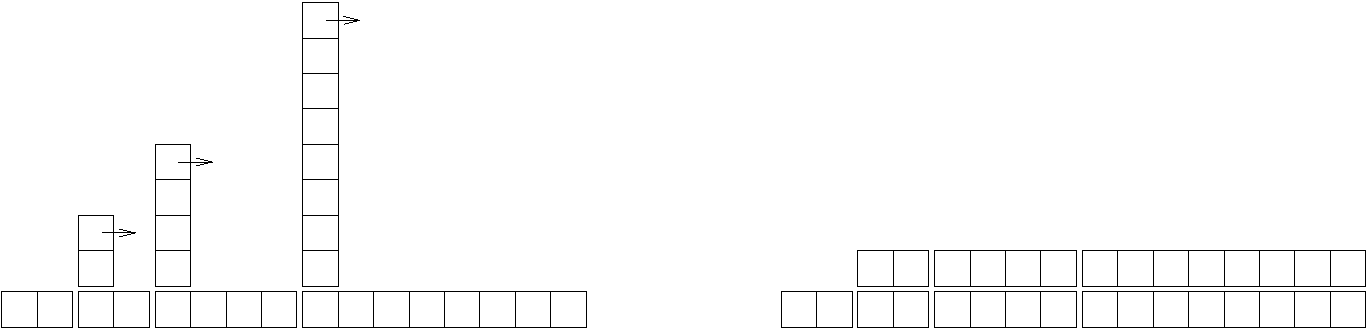
\includegraphics[width=5.5in]{../source/figs/towers.pdf}}
\caption{The cost of a hashtable add.\label{fig.hash}}
\end{figure}

The extra work of rehashing appears as a sequence of increasingly
tall towers with increasing space between them.  Now if you knock
over the towers, spreading the cost of resizing over all
adds, you can see graphically that the total cost after $n$
adds is $2n - 2$.

重哈希的额外工作显示为一序列增加的高塔并在它们之间增加空间。
现在,如果你打翻这些塔,将 resize 的代价均摊到所有的 add 上,
你会从图上看到 $n$ 个add的整个花费是 $2n - 2$ 。

An important feature of this algorithm is that when we resize the
HashTable it grows geometrically; that is, we multiply the size by a
constant.  If you increase the size
arithmetically---adding a fixed number each time---the average time
per {\tt add} is linear.

该算法一个重要的特征是当我们 resize 哈希表的时候,
它几何级增长。也就是说,我们用常数乘以大小。
如果你按算术级增加大小 —— 每次增加固定的数目—每个 \li{add} 的平均时间是线性的。
\index{geometric resizing}

You can download my implementation of HashMap from
\url{http://thinkpython2.com/code/Map.py}, but remember that there
is no reason to use it; if you want a map, just use a Python dictionary.

你可以 \href{http://thinkpython2.com/code/Map.py}{在此下载} 到 HashMap 的实现代码, 但在实际环境中直接使用 Python 的{\em 字典}足矣。

\section{Glossary  |  术语表}

\begin{description}

\item[]

\item[analysis of algorithms:] A way to compare algorithms in terms of
their run time and/or space requirements.

\item[算法分析] 比较不同算法间运行时间和资源占用的分析方法。
\index{analysis of algorithms}

\item[machine model:] A simplified representation of a computer used
to describe algorithms.

\item[模型机器] 用于描述算法(性能)的简化的计算机表示。
\index{machine model}

\item[worst case:] The input that makes a given algorithm run slowest (or
require the most space.

\item[最坏情况] 对给定算法话最长时间运行(或占用做多资源)的输入。
\index{worst case}

\item[leading term:] In a polynomial, the term with the highest exponent.

\item[首项] 在多项式中,拥有指数最高的项
\index{leading term}

\item[crossover point:] The problem size where two algorithms require
the same run time or space.

\item[交叉点] 两个算法对求解给定问题在某个规模需要相同运行时间或资源开销。
\index{crossover point}

\item[order of growth:] A set of functions that all grow in a way
considered equivalent for purposes of analysis of algorithms.
For example, all functions that grow linearly belong to the same
order of growth.

\item [增长阶数] 一些函数的组合,其函数值的增长在某种程度上等同于算法分析考察的目标。 例如, 线性递增的所有的函数都 属于 同一个增长阶数。
\index{order of growth}

\item[Big-Oh notation:] Notation for representing an order of growth;
for example, $O(n)$ represents the set of functions that grow
linearly.

\item[大O符号] 代表增长阶数的符号;例如, $O(n)$ 代表线性递增的函数。
\index{Big-Oh notation}

\item[linear:] An algorithm whose run time is proportional to
problem size, at least for large problem sizes.

\item[线性级] 算法的运行时间和所求解问题的规模成比例, 至少是在问题规模较大时显现。 
\index{linear}

\item[quadratic:] An algorithm whose run time is proportional to
$n^2$, where $n$ is a measure of problem size.

\item[二次方级] 算法的运行时间和说求解问题的规模的二次方($n^2$)成比例,$n$ 用于描述问题的规模。
\index{quadratic}

\item[search:] The problem of locating an element of a collection
(like a list or dictionary) or determining that it is not present.

\item[检索] 定位一个集合(例如列表或字典)中某个元素位置的问题,也等价于确认某元素不再该集合中的问题。
\index{search}

\item[hashtable:] A data structure that represents a collection of
key-value pairs and performs search in constant time.

\item[哈希表] 一种数据结构用于描述 键-值对 的集合,在该类集合运行检索任务只花费固定的时间(不依赖于集合的大小)。
\index{hashtable}

\end{description}
